\documentclass[fontsize=12pt,openright,oneside,paper=a4,BCOR=1cm]{scrbook}


\newcommand{\authorname}{Felix, Wilhelm}
\newcommand{\immatriculationnumber}{78186}
\newcommand{\studypath}{Internet Computing}
\newcommand{\currentsemester}{14}
\newcommand{\email}{wilhel40@ads.uni-passau.de}
\newcommand{\worktitle}{Prozessdesign- und Digitalisierung für eine moderne Wasserwachtverwaltung}
\newcommand{\thesistype}{Bachelorarbeit}
\newcommand{\thesisdate}{20.04.2022}
\newcommand{\thesisprof}{Prof. Harald Kosch}
\newcommand{\faculty}{Fakultät für Informatik und Mathematik}
\newcommand{\chair}{Lehrstuhl für Informatik mit Schwerpunkt Verteilte Informationssysteme}
\newcommand{\semester}{14}


%%%%%%%%%%%%%%%%%%%%%%%%%%%%%%%%%%%%%%%%%%%%%%%%%%%%%%%%%%%%

% PACKAGES:


% Use list of tabels, etc. in table of contents:
\usepackage{tocbibind}
% German paragraph skip
\usepackage{parskip}
% Encoder:????
\usepackage[utf8]{inputenc}
% Index-generation
\usepackage{makeidx}
% Einbinden von URLs:
\usepackage{url}
% Include .eps-files (needed also for the CNACC-logo):
\usepackage{epsf}
% Special \LaTex symbols (e.g. \BibTeX):
\usepackage{doc}
% Include Graphic-files:
%\usepackage{graphics}
% Include Graphic-files:
\usepackage{graphicx}
\usepackage{float}
% Include doc++ generated tex-files:
%\usepackage{docxx}
% Include PDF links
\usepackage{cite}
% Include citations
\usepackage{booktabs}
\usepackage{enumerate}
% figures
\usepackage{subcaption}

%mathstuff
\usepackage[cmex10]{amsmath}
\usepackage{amsfonts}
\usepackage{amssymb}

%hyperref for nice PDF output
\usepackage[pdftex, bookmarks=true]{hyperref}
\usepackage{pdfpages}

%%%%%%%%%%%%%%%%%%%%%%%%%%%%%%%%%%%%%%%%%%%%%%%%%%%%%%%%%%%%

% OTHER SETTINGS:

% Pagestyle:
\pagestyle{headings}

% Chapter Format:
\addtokomafont{chapter}{\Large}
\RedeclareSectionCommand[%
  beforeskip=12pt,
  afterskip=3pt 
]{chapter}

% Avoid 'overhang':
\sloppy

% Choose language
\newcommand{\setlang}[1]{\selectlanguage{#1}\nonfrenchspacing}

\usepackage[german]{babel}


\setlang{german}

%%%%%%%%%%%%%%%%%%%%%%%%%%%%%%%%%%%%%%%%%%%%%%%%%%%%%%%%%%%%

% TITLE:

\begin{document}

%\thispagestyle{empty}
%\newpage

\vspace{1cm}

\begin{center}
\begin{tabular}{lr}

\includegraphics[width=6.5cm]{logouni.pdf}
\end{tabular}

\vspace{1.0cm}
\Large Universität Passau
\\
\Large \faculty
\\
\vspace{0.3cm}
\large \chair
\\
\vspace{0.3cm}
\large Betreuer: \thesisprof
\\


\end{center}


\vspace{1.5cm}

\begin{center}
        {\Huge \worktitle } % Master Thesis, Programming Project
\end{center}
\vspace{1.5cm}
\begin{center}

        {\LARGE Bachelorarbeit}
        \\
        {\large
        \vspace{0.3cm}
        }
        {\large
        \vspace{0.1cm}
        \thesisdate
        }
\end{center}

\vspace{0.8cm}



\vfill {% \settowidth{\baselineskip}{0.2cm}

\vfill


{\normalsize
\begin{tabular}[l]{llll}
Name:     &  \authorname \\
Matrikelnummer:       & \immatriculationnumber \\
Fachsemester:       & \currentsemester \\
Studiengang:       & \studypath \\
E-Mail Adresse:       & \email \\
\smallskip \\

\end{tabular}}
} \cleardoublepage

%%%%%%%%%%%%%%%%%%%%%%%%%%%%%%%%%%%%%%%%%%%%%%%%%%%%%%%%%%%%


% MAIN PART:

% Inhaltsverzeichnis:
\tableofcontents

%%%%%%%%%%%%%%%%%%%%%%%%%%%%%%%%%%%%
%
% Kapitel 1
%
%%%%%%%%%%%%%%%%%%%%%%%%%%%%%%%%%%%%

\chapter{Einleitung}
\section{Hintergrund und Relevanz des Themas}
Die fortschreitende Digitalisierung und Automatisierung von Verwaltungsprozessen hat in den letzten Jahren auch vor gemeinnützigen Organisationen nicht haltgemacht. Insbesondere im Bereich der Wasserwacht, die sich der Rettung von Menschenleben in und um Gewässer widmet, eröffnen moderne Informationstechnologien neue Möglichkeiten, die Effizienz von Verwaltungstätigkeiten zu steigern. Im Rahmen meiner Bachelorarbeit habe ich mich mit diesem Thema auseinandergesetzt und eine Webanwendung entwickelt, um die Verwaltungsprozesse der Wasserwacht Dingolfing-Landau zu digitalisieren. 
\\
\section{Zielsetzung der Arbeit}
Das Ziel dieser Arbeit ist es, die Herausforderungen bei der Wachplanerstellung zu identifizieren und durch den Einsatz von IT-Lösungen zu bewältigen. Dabei wird insbesondere der Prozess der Wachplanung betrachtet, der eine essenzielle Rolle in der Organisation der Wasserwacht einnimmt. Traditionell werden Wachpläne manuell erstellt, was mit einem erheblichen Zeitaufwand und administrativem Aufwand verbunden ist. Durch den Einsatz einer Webanwendung sollen diese Prozesse vereinfacht und effizienter gestaltet werden, um Zeit und Ressourcen einzusparen. 
\\
\section{Methodik und Vorgehensweise}
Im Rahmen dieser Arbeit werde ich die Anforderungen an die Webanwendung analysieren, die Technologien zur Umsetzung auswählen und die Funktionalitäten der Anwendung im Detail erläutern. Dabei werden auch Aspekte wie Datensicherheit und Benutzerfreundlichkeit berücksichtigt. Die Evaluation der entwickelten Webanwendung erfolgt anhand von Nutzertests und Feedback der Wasserwachtmitglieder, um die Praxistauglichkeit und Effektivität der Anwendung zu überprüfen. 
\\
Die vorliegende Arbeit trägt somit zur Verbesserung der Verwaltungsprozesse in der Wasserwacht bei und liefert einen Beitrag zur Nutzung moderner Informationstechnologien im gemeinnützigen Bereich. Es wird erwartet, dass die entwickelte Webanwendung die Planung und Organisation von Wacheinsätzen erleichtert und somit zur Optimierung der Einsatzbereitschaft der Wasserwacht beiträgt. 
\\


%%%%%%%%%%%%%%%%%%%%%%%%%%%%%%%%%%%%
%
% Kapitel 2
%
%%%%%%%%%%%%%%%%%%%%%%%%%%%%%%%%%%%%

%TODO
\chapter{Theoretischer Hintergrund}

\section{Wasserwacht als gemeinnützige Organisation}

Die Wasserwacht ist eine gemeinnützige Organisation, die sich dem Schutz und der Sicherheit von Menschen im Wasser widmet. Als Teil des Deutschen Roten Kreuzes (DRK) setzt sie sich aus ehrenamtlichen Helfern und Fachkräften zusammen und spielt eine entscheidende Rolle bei der Gewährleistung der Wasserrettung und des Katastrophenschutzes. \\
Die Hauptaufgabe der Wasserwacht besteht darin, das Wohl und die Sicherheit von Menschen in Gewässern zu gewährleisten. Sie ist insbesondere in Seen, Flüssen, Schwimmbädern und Küstengebieten präsent und übernimmt wichtige Funktionen wie die Überwachung von Badebereichen, die Durchführung von Rettungsmaßnahmen und die Erste Hilfe bei Wasserunfällen. Die Wasserwacht ist darauf spezialisiert, in Notfällen schnell und effektiv zu reagieren und Menschenleben zu retten. \\
Neben der unmittelbaren Wasserrettung engagiert sich die Wasserwacht auch in der Prävention und Aufklärung. Sie organisiert Schwimmkurse, informiert über Gefahren im Wasser und beteiligt sich an Aktionen zur Förderung der Schwimmfähigkeit und Sicherheit im Wasser. Durch diese Aktivitäten trägt die Wasserwacht dazu bei, Unfälle zu vermeiden und das Bewusstsein für den verantwortungsvollen Umgang mit Wasser zu schärfen. \\
Als gemeinnützige Organisation ist die Wasserwacht auf die Unterstützung von Freiwilligen und Spenden angewiesen. Die ehrenamtlichen Helfer der Wasserwacht investieren ihre Zeit und ihr Engagement, um anderen Menschen in Notsituationen zu helfen und die Sicherheit in Gewässern zu gewährleisten. Sie absolvieren eine fundierte Ausbildung in Erster Hilfe, Rettungstechniken und Kommunikation, um bestmöglich auf Einsätze vorbereitet zu sein. \\
Die Wasserwacht ist eng mit lokalen Gemeinschaften verbunden und arbeitet oft eng mit anderen Rettungsorganisationen, wie beispielsweise der Feuerwehr oder der DLRG, zusammen. Sie spielt eine wichtige Rolle bei der Bewältigung von Notfällen und Katastrophen, sei es bei Naturkatastrophen oder bei Großveranstaltungen in der Nähe von Gewässern. \\
Insgesamt ist die Wasserwacht eine essentielle gemeinnützige Organisation, die sich unermüdlich für die Sicherheit und das Wohlergehen von Menschen im Wasser einsetzt. Ihr Engagement, ihre Fachkenntnisse und ihre Einsatzbereitschaft machen sie zu einer vertrauenswürdigen Institution, die maßgeblich dazu beiträgt, Unfälle zu verhindern und Leben zu retten.

\section{Verwaltungsprozesse in der Wasserwacht}

Die Wasserwacht ist nicht nur für die Wasserrettung und den Katastrophenschutz zuständig, sondern auch mit einer Reihe von Verwaltungsprozessen betraut, um einen reibungslosen Ablauf ihrer Aufgaben und Aktivitäten sicherzustellen. Diese Verwaltungsprozesse sind von großer Bedeutung, da sie die organisatorische Struktur und das Funktionieren der Wasserwacht unterstützen.\\
Ein wesentlicher Verwaltungsprozess in der Wasserwacht ist die Dokumentation und Verwaltung der Mitgliederinformationen. Die Wasserwacht ist oft in einem größeren geografischen Gebiet tätig und hat zahlreiche Mitglieder, die über verschiedene Standorte verteilt sein können. Es ist wichtig, die relevanten Informationen zu den Mitgliedern, wie Kontaktdaten, Qualifikationen, Ausbildungsstand oder Verfügbarkeiten, zu erfassen und zu verwalten. Dies ermöglicht eine effektive Kommunikation, Koordination und Einsatzplanung. \\
Ein weiterer wichtiger Verwaltungsprozess ist die Einsatz- und Wachplanung. Die Wasserwacht ist regelmäßig in der Gewässerüberwachung und Rettungseinsätzen involviert. Die Planung und Organisation dieser Einsätze erfordert eine genaue Koordination der verfügbaren Ressourcen, wie Wachkräfte, Rettungsmittel oder Sanitätsausrüstung. Die Wasserwacht muss sicherstellen, dass zu jeder Zeit ausreichend qualifizierte Kräfte anwesend sind, um auf Notfälle reagieren zu können. Die Verwaltung dieser Planung kann zeitaufwändig sein, insbesondere wenn sie manuell oder auf papierbasierten Systemen durchgeführt wird. \\
Des Weiteren umfasst die Verwaltung in der Wasserwacht auch die Erfassung und Auswertung von Daten und Statistiken. Dies beinhaltet beispielsweise die Erfassung von Einsatzzahlen, Schwimmprüfungen, Ausbildungsnachweisen oder Protokollen. Die Analyse dieser Daten ermöglicht es der Wasserwacht, Trends zu erkennen, ihre Leistung zu bewerten und die Planung zukünftiger Aktivitäten zu verbessern. \\
Ein effizientes Management von Materialbeständen und Ausrüstung ist ebenfalls Teil der Verwaltungsprozesse. Die Wasserwacht benötigt eine Vielzahl von Rettungsmitteln, Sanitätsausrüstung und weiterem Material, um ihre Aufgaben erfüllen zu können. Die Verwaltung dieser Bestände, einschließlich der Überwachung von Lagerbeständen, der Beschaffung und Wartung von Ausrüstung sowie der Inventarisierung, ist entscheidend, um sicherzustellen, dass die Wasserwacht jederzeit über die erforderlichen Ressourcen verfügt. \\
Insgesamt sind die Verwaltungsprozesse in der Wasserwacht unerlässlich, um einen geordneten und effizienten Betrieb zu gewährleisten. Die Digitalisierung und Automatisierung dieser Prozesse kann dazu beitragen, Zeit und Ressourcen zu sparen, Fehler zu minimieren und die Kommunikation und Koordination innerhalb der Organisation zu verbessern. Die Entwicklung einer Webanwendung zur Verwaltung dieser Prozesse, wie beispielsweise der Wachplanerstellung, kann einen bedeutenden Fortschritt bei der Modernisierung und Effizienzsteigerung der Wasserwacht bedeuten.

\section{Herausforderungen bei der Wachplanerstellung}

Die Wachplanerstellung in der Wasserwacht stellt eine Reihe von Herausforderungen dar, die es zu bewältigen gilt. Ein effizienter und gut durchdachter Wachplan ist von entscheidender Bedeutung, um sicherzustellen, dass zu jeder Zeit ausreichend qualifizierte Kräfte für die Gewässerüberwachung und Rettungseinsätze zur Verfügung stehen. Im Folgenden werden einige der Hauptprobleme und Herausforderungen bei der Wachplanerstellung in der Wasserwacht erläutert:

    Verfügbarkeit der Helfer: Die Wasserwacht ist in erster Linie auf die Unterstützung von ehrenamtlichen Helfern angewiesen. Diese Helfer haben jedoch oft andere Verpflichtungen wie Beruf, Studium oder Familie, die ihre Verfügbarkeit beeinflussen können. Die Herausforderung besteht darin, den Wachplan so zu gestalten, dass er die Verfügbarkeit der Helfer berücksichtigt und sicherstellt, dass zu jeder Zeit ausreichend Kräfte vor Ort sind.

    Qualifikationen und Ausbildungsstand: Für die Wachplanerstellung ist es wichtig, die Qualifikationen und den Ausbildungsstand der Helfer zu berücksichtigen. Je nach Art der Wasserrettungseinsätze und Gewässerbedingungen können bestimmte Fähigkeiten und Zertifizierungen erforderlich sein. Die Herausforderung besteht darin, den Wachplan so zu erstellen, dass qualifizierte Helfer an den richtigen Stellen eingesetzt werden und die Sicherheitsstandards gewährleistet sind.

    Flexibilität und Änderungen: Der Wachplan muss flexibel genug sein, um Änderungen und unvorhergesehene Ereignisse zu berücksichtigen. Dies können beispielsweise kurzfristige Absagen von Helfern, unvorhergesehene Ereignisse oder Änderungen in den Einsatzanforderungen sein. Die Herausforderung besteht darin, den Wachplan so zu gestalten, dass er leicht anpassbar ist und dennoch eine kontinuierliche Gewässerüberwachung gewährleistet.

    Kommunikation und Koordination: Die Wachplanerstellung erfordert eine effektive Kommunikation und Koordination innerhalb der Wasserwacht. Informationen über Verfügbarkeiten, Änderungen und Einsatzanforderungen müssen schnell und zuverlässig zwischen den Verantwortlichen ausgetauscht werden. Die Herausforderung besteht darin, sicherzustellen, dass die Kommunikation reibungslos verläuft und alle relevanten Informationen zeitnah zur Verfügung stehen.

    Fairness und Ausgewogenheit: Bei der Wachplanerstellung ist es wichtig, Fairness und Ausgewogenheit sicherzustellen. Dies bedeutet, dass die Arbeitsbelastung gerecht auf die Helfer verteilt wird und jeder die Möglichkeit hat, sich einzubringen. Die Herausforderung besteht darin, den Wachplan so zu erstellen, dass er diesen Grundsätzen gerecht wird und gleichzeitig den Anforderungen der Wasserwacht entspricht.

Die Wachplanerstellung in der Wasserwacht ist eine komplexe Aufgabe, die sorgfältige Planung, Koordination und Berücksichtigung verschiedener Faktoren erfordert. Durch den Einsatz moderner Technologien wie einer Webanwendung können viele dieser Herausforderungen bewältigt und die Effizienz bei der Wachplanerstellung gesteigert werden. Eine gut konzipierte und durchdachte Lösung kann dazu beitragen, die Wachplanung zu optimieren und einen reibungslosen Ablauf der Gewässerüberwachung und Rettungseinsätze zu gewährleisten.

\section{Bedeutung von IT-Lösungen zur Digitalisierung von Verwaltungsprozessen} 

Die Bedeutung von IT-Lösungen zur Digitalisierung von Verwaltungsprozessen ist in der heutigen Zeit von großer Relevanz. Traditionell wurden Verwaltungsprozesse in vielen Organisationen, einschließlich der Wasserwacht, manuell oder mit papierbasierten Systemen abgewickelt. Dies führte häufig zu ineffizienten Abläufen, einer hohen Fehleranfälligkeit und einem erheblichen Zeitaufwand.

Die Einführung von IT-Lösungen zur Digitalisierung von Verwaltungsprozessen bietet zahlreiche Vorteile. Ein zentraler Aspekt ist die Automatisierung von Aufgaben und die Reduzierung manueller Eingriffe. Durch den Einsatz von speziell entwickelten Webanwendungen oder Softwarelösungen können Verwaltungsprozesse optimiert und beschleunigt werden. Die erforderlichen Informationen können elektronisch erfasst, gespeichert und bearbeitet werden, was zu einer erheblichen Zeitersparnis führt.

Darüber hinaus ermöglichen IT-Lösungen eine verbesserte Datenverwaltung und -analyse. Durch die Digitalisierung von Verwaltungsprozessen können Daten effizient erfasst, organisiert und ausgewertet werden. Dies ermöglicht es der Wasserwacht, wertvolle Erkenntnisse zu gewinnen, Trends zu erkennen und fundierte Entscheidungen zu treffen. Beispielsweise können Einsatzstatistiken, Mitgliederdaten oder Materialbestände elektronisch erfasst und in Echtzeit analysiert werden, um einen umfassenden Überblick zu erhalten.

Des Weiteren führt die Digitalisierung von Verwaltungsprozessen zu einer verbesserten Kommunikation und Zusammenarbeit. Durch den Einsatz von IT-Lösungen können Informationen schnell und zuverlässig zwischen den relevanten Personen und Abteilungen ausgetauscht werden. Dies erleichtert die Koordination von Aufgaben, die Planung von Einsätzen und die effektive Zusammenarbeit. Durch den Zugriff auf gemeinsame Datenbanken oder Kollaborationstools können Informationen in Echtzeit geteilt werden, was zu einer erhöhten Effizienz und Transparenz führt.

Nicht zuletzt tragen IT-Lösungen zur Digitalisierung von Verwaltungsprozessen auch zur Verbesserung der Servicequalität bei. Durch den Einsatz von automatisierten Prozessen und einem benutzerfreundlichen Interface können Verwaltungsaufgaben effizienter erledigt werden. Dies ermöglicht es der Wasserwacht, ihre Ressourcen effektiver einzusetzen und sich auf ihre Kernaufgaben, wie die Wasserrettung und den Katastrophenschutz, zu konzentrieren. Gleichzeitig können die Mitglieder der Wasserwacht von einer vereinfachten Kommunikation und einer besseren Organisation profitieren.

Insgesamt ist die Bedeutung von IT-Lösungen zur Digitalisierung von Verwaltungsprozessen in der Wasserwacht nicht zu unterschätzen. Die Einführung solcher Lösungen ermöglicht eine effizientere Arbeitsweise, eine verbesserte Datenverwaltung und -analyse, eine gesteigerte Zusammenarbeit sowie eine höhere Servicequalität. Die Digitalisierung von Verwaltungsprozessen bietet somit eine bedeutende Chance für die Wasserwacht, ihre Abläufe zu optimieren und ihre Leistungsfähigkeit zu steigern.

\section{Best Practises Websitedesign}

%Hier auf DesignMetriken eingehen, Usability, Accessability, Cost, Delay,... 
% In Kapitel 5 darauf eingehen, wie man die Punkte erreicht. 


%TODO

%%%%%%%%%%%%%%%%%%%%%%%%%%%%%%%%%%%%
%
% Kapitel 3
%
%%%%%%%%%%%%%%%%%%%%%%%%%%%%%%%%%%%%

\chapter{Anforderungsanalyse}
\section{Identifikation von Anforderungen an die Webanwendung} 
Bevor mit der eigentlichen Implementierung der Anwendung gestartet werden kann, müssen zunächst die Anforderungen daran festgemacht werden. \\
In einem initial bereitgestelltem Dokument (siehe Anhang ~\ref{fig:initial}) sind die ersten Entwürfe der Anwendung aufgezeichnet. Darin sieht man mehrere gewünschte Features, um die Verwaltungsarbeiten der Wasserwacht abzudecken, wie beispielsweise "Wachplanung", "Materialcheck", "Wachbuch" oder "Sanitätsbuch". In dieser Arbeit werden hauptsächlich die Punkte "Wachplanung" und "Wachbuch" ausgearbeitet, welche im folgenden detaillierter beschrieben werden. \\ 

\subsection{Nutzergruppen}
Für die Anwendung werden zwei Nutzergruppen angefordert. \\
Zunächst hat man die "Leitungskräfte / Admins". Diese sind für administrative Tätigkeiten zuständig und erledigen die Planung und Verwaltung der Anwendung. 
Außerdem gibt es noch die "Mitglieder / Helfer". Diese spielen vor Allem bei der Durchführung der jeweiligen Wachtage eine Rolle.

\subsection{Wachplanung}
Leitungskräften soll es ermöglicht werden im Voraus Termine für die einzelnen Wachpläne einzustellen. Diese sollen für ein konkretes Datum und Uhrzeit erstellt werden können, oder als Serie mit einer bestimmten Laufzeit. In einem Kalender sollen die einzelnen Termine dargestellt werden, mit einer farblichen Kennung, ob für diesen Termin bereits Mitarbeiter eingebucht sind. \\
Für Mitglieder ist es notwendig, sich für Wachtage einzubuchen. Dazu soll auch der Kalender genutzt werden, um eine Übersicht der verfügbaren Wachtage zu erhalten.

\subsection{Wachbuch}
Im Wachbuch werden die Ereignisse eines Wachtages festgehalten. Nutzern soll es möglich sein, eine Liste der gebuchten Helfern anzuzeigen, sowie nach Wachstart eine Liste der anwesenden Helfern anzuzeigen. Nutzer können sich für diesen Wachtag ein-, bzw. ausbuchen. \\
Weiterhin werden für diesen Wachtag die vorliegenden Wetterdaten vorliegen, welche über eine API ermittelt werden. Nutzer können die aktuelle Wassertemperatur über ein Eingabefeld abspeichern. \\
Die Ereignisse des Wachtags werden in einer Tabelle, mit Namen und Zeitstempel, festgehalten. Dabei werden der Wachbeginn und das Wachende der Mitglieder, die An- und Abmeldung im ILS, die automatischen Wetterdaten und der Wachstart/ -ende automatisch eingetragen. Nutzer können zusätzlich manuell Eingaben tätigen. \\
Leitungskräften soll es zusätzlich ermöglicht werden eine Auswertung eines Wachtages vorzunehmen. Dazu gibt es einen Button "Drucken", über den ein PDF, welches die Ereignisse des Wachtages zusammenfasst, heruntergeladen werden kann. Die Informationen, welche dieses Dokument enthalten muss, wurden aus einem derzeit verwendeten Wachbuch übernommen (siehe Anhang ~\ref{fig:wachbuchpapier}). Darin befinden sich die vorliegenden Wetterdaten, Informationen über das anwesende Wachpersonal, sowie das Wachtagebuch. \\
Die Punkte "Übersicht Checks" und "Einsätze" wurden im Rahmen dieser Arbeit aus zeitlichen Gründen nicht betrachtet. 

\section{Befragung von Wasserwachtmitgliedern und Mockups}
In mehreren Iterationen wurden mit Herrn Andreas Schmeisl (Vorsitzender Kreiswasserwacht Dingolfing-Landau) und Herrn Werner Gerl (Technischer Leiter) die finalen Vorgaben geklärt. Dabei wurde mit Hilfe von Mockups ein Zielbild der Anwendung entwickelt. 
\subsection{Mockups}
\subsubsection{Was sind Mockups}
%Definition Mockups, warum werden sie in der Planung von Software eingesetzt
Mockups werden in der Softwareentwicklung eingesetzt um sicher zu gehen, dass man die Anforderungen an die Anwendung verstanden hat. Mockups haben den Vorteil, dass sie kosten- und zeiteffizient erstellt werden können und schnell anpassbar sind.

\subsubsection{Papier-Mockups}
In einem initialen Meeting wurden mit Papier Mockups die groben Umrisse der Website aufgezeigt. Es wurden außerdem noch weitere Funktionalitäten und Anforderungen besprochen, die aus den vorliegenden Unterlagen nicht hervorgingen. \\
Mit den Ergebnissen aus diesem Meeting konnte ein Prototyp der Anwendung erstellt werden.


\subsubsection{Figma}
%Website beschreiben 
Figma ist eine Website, über die man Protoypen und Mockups erstellen kann. Über einzelne Boards können die verschiedenen Seiten der Zielanwendung simuliert werden. Der Vorteil hierbei ist, dass auch Nutzereingaben simuliert werden können. So kann beispielsweise bei Klicken ein Seitensprung animiert werden. Dadurch kann man ohne viel Aufwand dem Kunden zeigen, wie die Anwendung einmal aussehen wird. 

\subsection{Ergebnisse}
%Bilder der Mocks darstellen, einzelne Masken wurden konkretisiert, weitere Anforderungen wurden aufgenommen, Emailversand bei Login. 
Mit Figma wurden alle vorgesehenen Seiten und Funktionalitäten der Website simuliert. Im folgenden werden die Ergebnisse und die weiteren besprochenen Anforderungen präsentiert. \\

\subsubsection{Anmeldeprozess}

Beim Login Prozess wurde gefordert, dass die "Admins" bei einer Neu-Anmeldung über Email benachrichtigt werden. Neue Nutzer können daher nach dem Registrieren nicht sofort auf die Seite zugreifen, sondern müssen erst warten bis ein Admin sie bestätigt hat. Dadurch soll sichergestellt werden, dass nur Wasserwachtmitglieder Zugang zum System erhalten.\\

\begin{figure}[H]
  \centering
  \begin{subfigure}[b]{0.4\linewidth}
    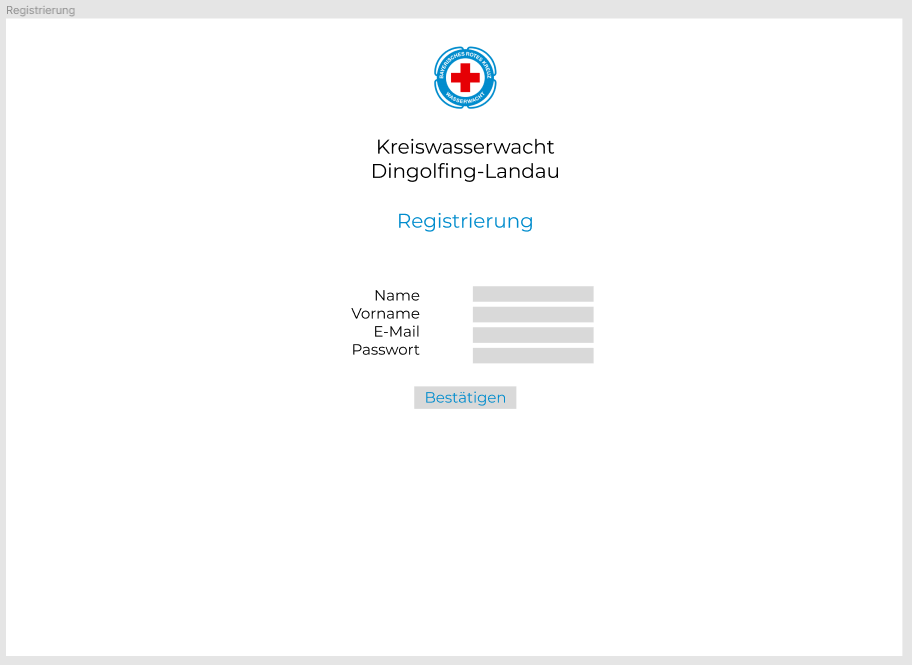
\includegraphics[width=\linewidth]{Anlagen/Figma/2-Registrierung.png}
    \caption{Registrierung}
  \end{subfigure}
  \begin{subfigure}[b]{0.4\linewidth}
    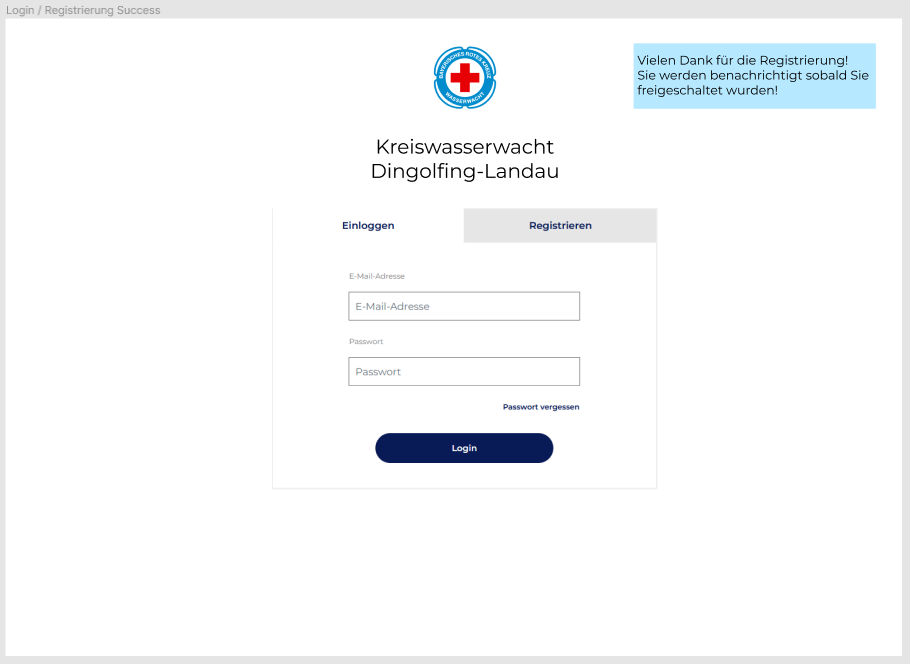
\includegraphics[width=\linewidth]{Anlagen/Figma/3-LoginSuccess.png}
    \caption{Benachrichtigung nach Registrierung}
  \end{subfigure}
  \caption{AnmeldeProzess}
  \label{fig:anmeldeprozess}
\end{figure}

%Nutzerübersicht
\subsubsection{Nutzerübersicht}

Admins sehen auf der Nutzerübersicht alle Nutzer und ob sie bereits freigeschaltet wurden. Über das jeweilige Nutzerprofil können sie den Nutzer über einen Button freischalten. Danach wird der Nutzer per Email benachrichtigt und erhält Zugang zum System. Außerdem soll für jeden Nutzer eine Statistik erhoben werden, wie viele Stunden im Dienst verbracht wurden. Dies wurde als Anforderung mit aufgenommen, wurde jedoch im Mock nicht mehr eingearbeitet sondern direkt in die tatsächliche Anwendung eingebaut.\\

\begin{figure}[H]
  \centering
  \begin{subfigure}[b]{0.4\linewidth}
    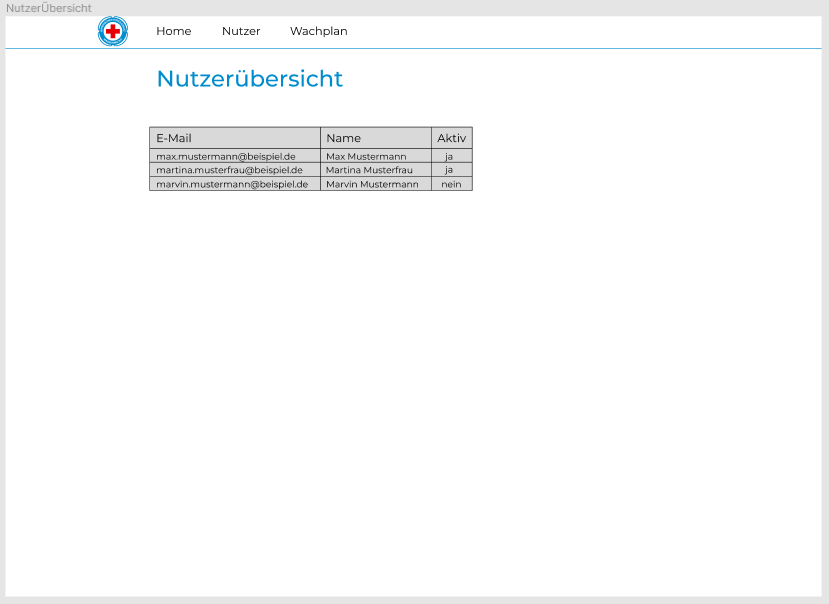
\includegraphics[width=\linewidth]{Anlagen/Figma/6-Nutzeruebersicht.png}
    \caption{Nutzerübersicht}
  \end{subfigure}
  \begin{subfigure}[b]{0.4\linewidth}
    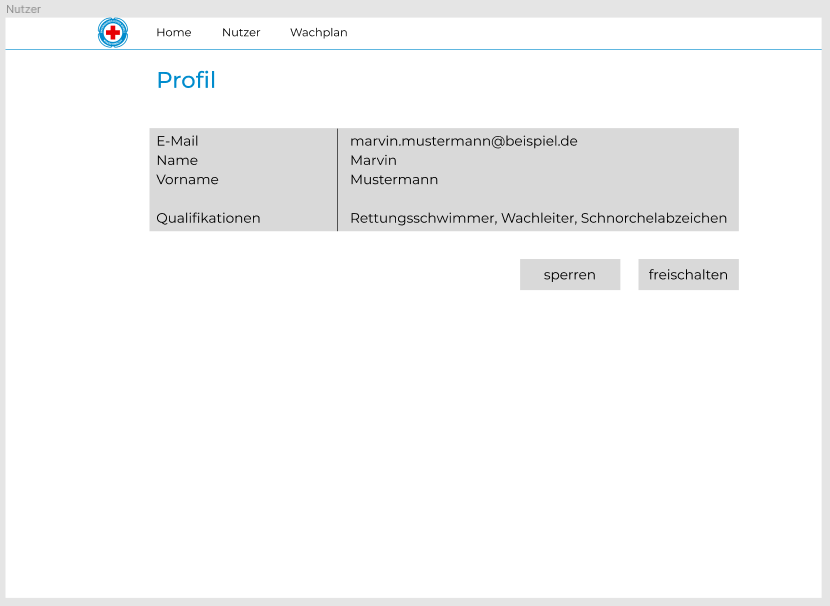
\includegraphics[width=\linewidth]{Anlagen/Figma/7-ProfilAdminSicht.png}
    \caption{Profil Admin Ansicht}
  \end{subfigure}
  \caption{Freischaltungs-Prozess}
  \label{fig:freischaltprozess}
\end{figure}

%Wachplan
\subsubsection{Wachplanung}

Bei der Wachplanung wurde angefordert, dass Wachtermine einzeln für ein bestimmtes Datum und Uhrzeit angelegt werden können. Außerdem soll es möglich sein gleich eine Reihe an Terminen anzulegen. Dazu muss ein Start- und Enddatum angegeben werden, die Uhrzeit, sowie die Wochentage an denen ein Termin eingestellt werden soll. \\
Als Übersicht für die bisherigen Termine wird ein Kalender verwendet. Hier wurde überlegt, ob man die einzelnen Termine farbig codiert, wenn beispielsweise ein "Rettungsschwimmer" und "Wachleiter" noch nicht eingebucht sind. In weiteren Abstimmungsterminen hat man sich aber darauf geeinigt, die Termine rot einzufärben, wenn noch niemand eingebucht ist, und grün einzufärben wenn Nutzer eingebucht sind (vgl. \cite[S. 49]{sklar2011principles}).

\begin{figure}[H]
  \centering
  \begin{subfigure}[b]{0.7\linewidth}
    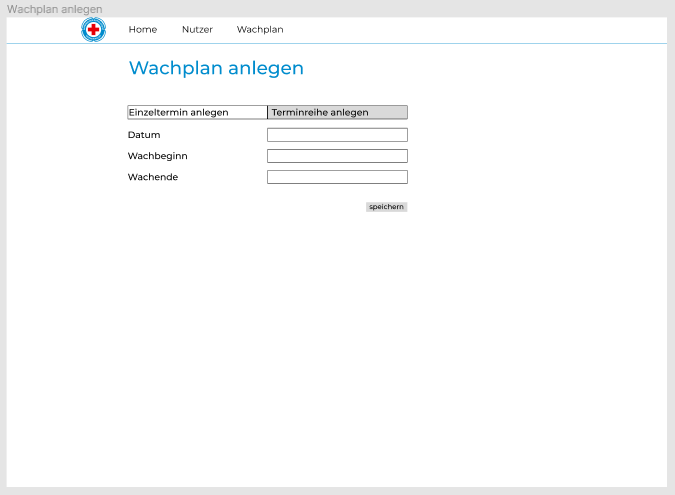
\includegraphics[width=\linewidth]{Anlagen/Figma/10-Wachplananlegen.png}
    \caption{Einzeltermin anlegen}
  \end{subfigure}
  \begin{subfigure}[b]{0.7\linewidth}
    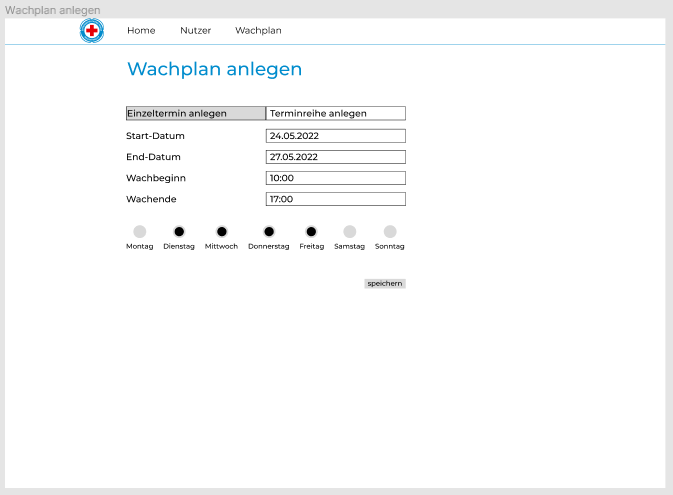
\includegraphics[width=\linewidth]{Anlagen/Figma/12-WachplanReiheAnlegenBef.png}
    \caption{Terminreihe anlegen}
  \end{subfigure}
  \begin{subfigure}[b]{0.7\linewidth}
    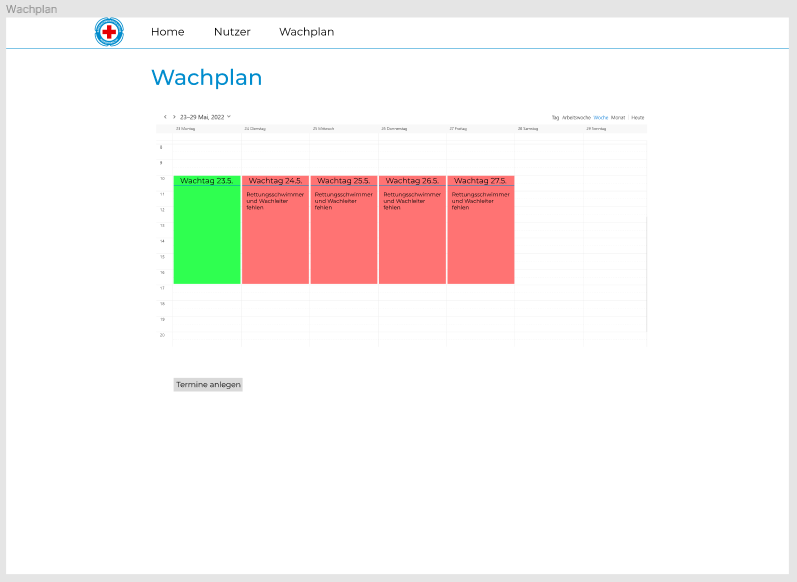
\includegraphics[width=\linewidth]{Anlagen/Figma/13-WachplanuebersichtAngelegt.png}
    \caption{Wachplan Übersicht}
  \end{subfigure}
  \caption{Wachplanung}
  \label{fig:wachplan}
\end{figure}

%Wachplandurchführung
\subsubsection{Wachplandurchführung}

Über einen Klick auf die Terminelemente im Wachplan kommt man auf die Durchführungsseite des jeweiligen Wachtages. Diese Seite wurde entsprechend der initialen Vorgabe (siehe Anhang ~\ref{fig:initial}) nachmodelliert. \\
Zunächst findet man oben auf der Seite das Tagesdatum, sowie die aktuelle Uhrzeit. Daneben findet man die Uhrzeit des Wachbeginn und Wachende. \\
Rechts oben befindet sich die Ausgabe der aktuellen Wetterdaten, welche automatisch eingespielt werden sollen. Hierfür wurde nach einer passenden Wetter-Anwendung gesucht, welche eine API zur Abfrage der Daten bereitstellt. Darunter befindet sich noch ein Eingabefeld für die aktuelle Wassertemperatur. Diese wird von Wasserwachtmitgliedern gemessen und im System hinterlegt. \\ 
Darunter befinden sich die Tabellen mit den Helfern für den Wachtag. Auf der linken Seite befindet sich die Tabelle mit den gebuchten Helfern. Ist ein Wachtag noch nicht gestartet, können sich Nutzer über ein darunter liegendes Eingabefeld einbuchen. Somit kann eine Planung der jeweiligen Wachtage stattfinden und man erhält einen Überblick, wie viele Personen planen vor Ort zu sein. Rechts daneben befindet sich die Tabelle der anwesenden Helfer. Sobald ein Wachtag gestartet wurde können sich die Nutzer über das gleiche Eingabefeld einbuchen und ihren Wachbeginn dokumentieren. Hier wurde in weiteren Besprechungen noch angefordert, dass es möglich sein soll Nutzer aus einer Auswahlliste auszuwählen und einzubuchen und zusätzlich auch über ein Freitextfeld einzugeben. Die Möglichkeit Nutzer über einen Freitext hinzufügen zu können wird benötigt, da auch Helfer am Dienst teilnehmen können, die nicht im System als Nutzer registriert sind. \\
Über den Button darunter kann eine An- und Abmeldung in der ILS (Integrierte Leitstelle) dokumentiert werden. Daneben befindet sich der Button zum starten und beenden eines Wachtages.\\
Darunter befindet sich ein größeres Texteingabefeld, wodurch Geschehnisse während des Wachtages festgehalten werden können im Wachbuch darunter. \\
Das Wachbuch enthält alle Ereignisse eines Wachtages. Ein Eintrag enthält immer einen Zeitstempel und den jeweiligen Nutzer der den Eintrag verfasst hat, bzw "System" wenn der Eintrag automatisch eingefügt wurde. Das Wachbuch dokumentiert somit Wachbeginn und Ende, Wachbeginn und Ende der jeweiligen Nutzer, die Wetterdaten, die Wassertemperatur, An- und Abmeldungen im ILS, sowie eigene Ereignisangaben der Nutzer.\\
Ein Feature das im Mock noch nicht dargestellt wurde ist das Drucken eines Wachtages. Nach Beendigung eines Wachtages soll es möglich sein die gesammelten Daten als PDF herunterzuladen. Dafür wurde ein Dokument bereitgestellt, welches aktuell benutzt wird um den Wachtag zu protokollieren. Nach dieser Vorlage soll auch das PDF erstellt werden mit den Daten aus dem System.

\begin{figure}[H]
  \centering
  \begin{subfigure}[b]{0.7\linewidth}
    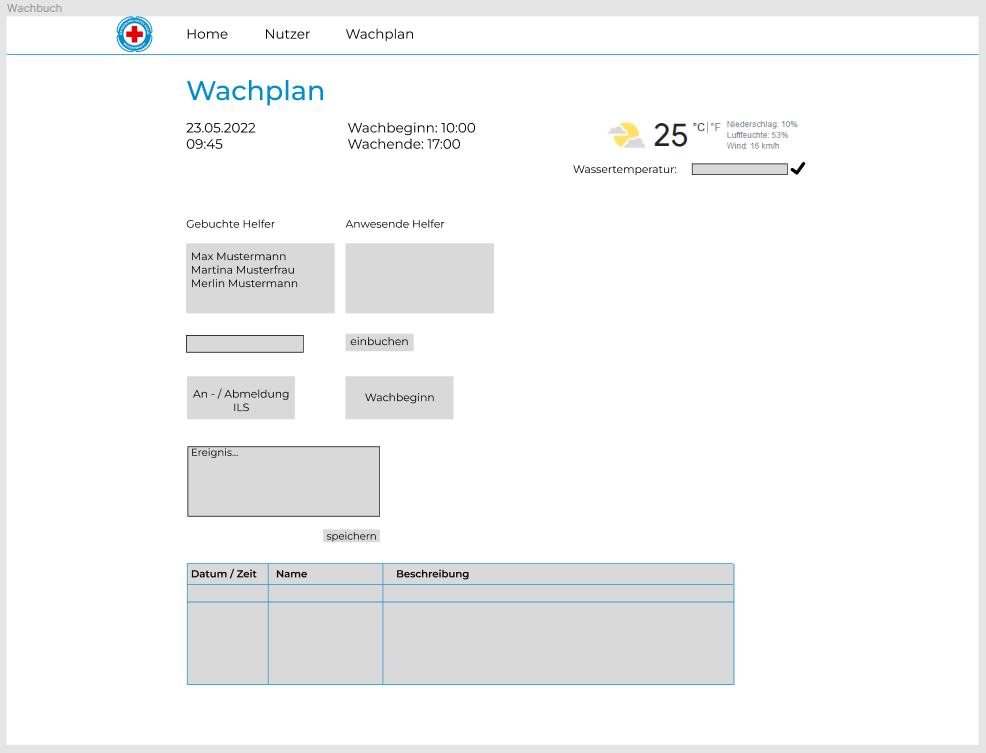
\includegraphics[width=\linewidth]{Anlagen/Figma/14-WachplanDurchfuehrung.png}
    \caption{Wachstart}
  \end{subfigure}
  \begin{subfigure}[b]{0.7\linewidth}
    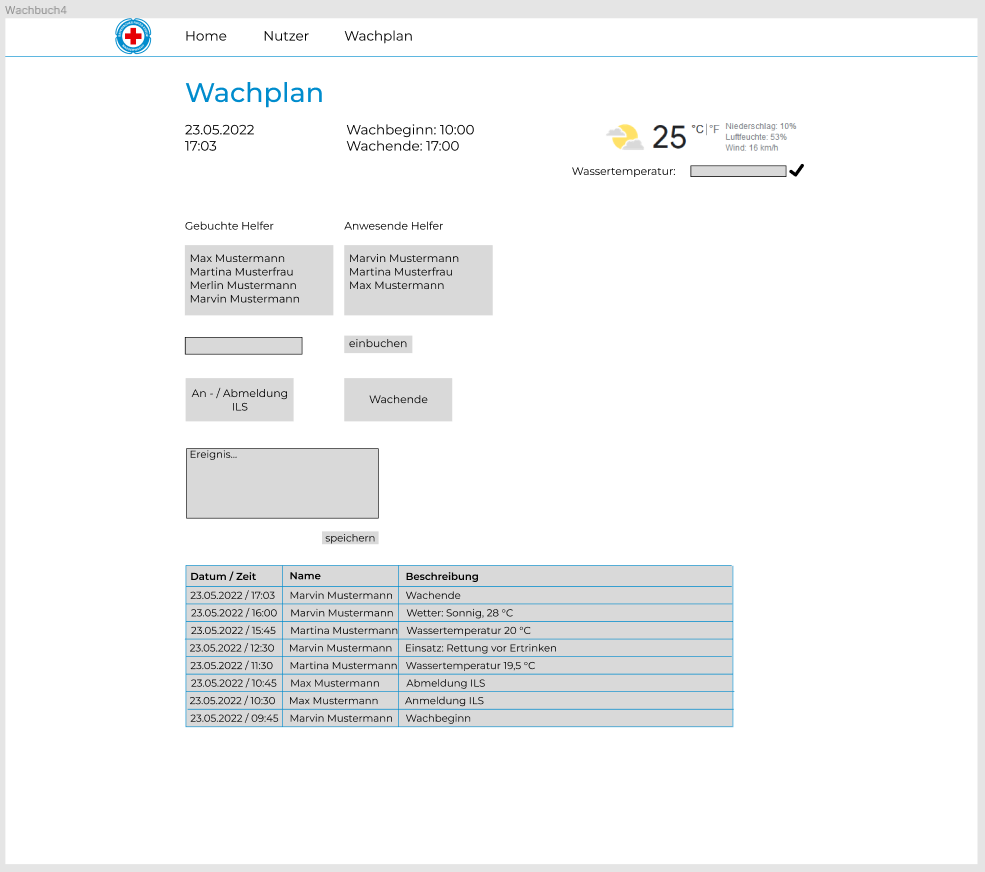
\includegraphics[width=\linewidth]{Anlagen/Figma/19-WachplanDurchfuehrung.png}
    \caption{Wachende}
  \end{subfigure}
  \caption{Wachbuch}
  \label{fig:wachbuch}
\end{figure}

%%%%%%%%%%%%%%%%%%%%%%%%%%%%%%%%%%%%
%
% Kapitel 4
%
%%%%%%%%%%%%%%%%%%%%%%%%%%%%%%%%%%%%
\renewcommand{\cleardoublepage}{}
\chapter{Technologien und Methoden}

Im folgenden Kapitel werden die verwendeten Technologien und Methoden der Entwicklung näher betrachtet und erläutert.

\section{Auswahl geeigneter Technologien und Tools für die Webanwendung}

Bei der Auswahl der Technologien und Tools für die Entwicklung meiner Webanwendung habe ich mich bewusst für Tools entschieden, mit denen ich bereits praktische Erfahrung sammeln konnte. Während meines Entwicklungspraktikums an der Universität habe ich mit den gleichen Tools gearbeitet, nämlich Java als Programmiersprache, das Spring-Framework für die Backend-Entwicklung, Thymeleaf für die serverseitige HTML-Vorlagenverarbeitung und Bootstrap für das Frontend-Design. Diese praktische Erfahrung ermöglichte mir einen reibungslosen Start in das Projekt, da ich bereits mit den Konzepten, Funktionalitäten und bewährten Methoden dieser Tools vertraut war. Durch die Verwendung von Java und den genannten Frameworks konnte ich eine solide und effiziente Entwicklungsumgebung schaffen, um die Anforderungen der Webanwendung erfolgreich umzusetzen.
Im folgenden werden die angewandten Technologien näher beschrieben.

\section{Beschreibung der verwendeten Programmiersprachen, Frameworks und Datenbanken}

\subsection{Spring}

\subsection{Thymeleaf}

\subsection{Bootstrap}

\subsection{Postgres}

\subsection{Wetter API}

\section{Agile Entwicklungsmethoden zur Umsetzung des Projekts}


%%%%%%%%%%%%%%%%%%%%%%%%%%%%%%%%%%%%
%
% Kapitel 5
%
%%%%%%%%%%%%%%%%%%%%%%%%%%%%%%%%%%%%

\renewcommand{\cleardoublepage}{}
\chapter{Konzeption und Umsetzung}

\section{Detaillierte Beschreibung der Konzeption der Webanwendung}

\subsection{Datenmodell}
\subsection{Prozesse}

\section{Funktionalitäten und Features der Anwendung}

\section{Umsetzung der Webanwendung anhand von Best Practises}


%%%%%%%%%%%%%%%%%%%%%%%%%%%%%%%%%%%%
%
% Kapitel 6
%
%%%%%%%%%%%%%%%%%%%%%%%%%%%%%%%%%%%%

\renewcommand{\cleardoublepage}{}
\chapter{Evaluation}

Um sicherzustellen, dass die Website den Anforderungen der Wasserwacht entspricht, wird im folgenden eine Evaluierung durchgeführt. Dies geschieht zunächst mit Nutzertest und Befragung von Wasserwachtmitgliedern. Weiterhin wird die Praxistauglichkeit und Effektivität der Webanwendung bewertet, mit den Punkten die in Kapitel 2.5 dargestellt wurden. Außerdem werden noch "Klickmetriken" betrachtet, für die zwei Haupt Anwendungsfälle. Abschließend wird daraus ein Fazit gezogen und auf Verbesserungspotentiale eingegangen. 

\section{Nutzertests und Feedback der Wasserwachtmitglieder}

\section{Bewertung der Praxistauglichkeit und Effektivität der Webanwendung}

%Hier Punkte aus 2 aufgreifen

\section{Klickmetriken}

\section{Verbesserungspotentiale}

%%%%%%%%%%%%%%%%%%%%%%%%%%%%%%%%%%%%
%
% Kapitel 7
%
%%%%%%%%%%%%%%%%%%%%%%%%%%%%%%%%%%%%

\renewcommand{\cleardoublepage}{}
\chapter{Ergebnisse und Diskussion}

\section{Zusammenfassung der Ergebnisse}

\section{Diskussion der Erkenntnisse im Kontext der Zielsetzung der Arbeit}

\section{Ausblick auf zukünftige Entwicklungen und mögliche Erweiterungen der Webanwendung}

%%%%%%%%%%%%%%%%%%%%%%%%%%%%%%%%%%%%
%
% Kapitel 8
%
%%%%%%%%%%%%%%%%%%%%%%%%%%%%%%%%%%%%

\renewcommand{\cleardoublepage}{}
\chapter{Fazit}

\section{Zusammenfassung der Arbeit}

\section{Beantwortung der Forschungsfrage}

\section{Schlussfolgerungen und Handlungsempfehlungen}

%%%%%%%%%%%%%%%%%%%%%%%%%%%%%%%%%%%%
%
% Anlagen
%
%%%%%%%%%%%%%%%%%%%%%%%%%%%%%%%%%%%%

\renewcommand{\cleardoublepage}{}

\begin{appendix}
\chapter{Anhang}
\section{Initialer Entwurf}

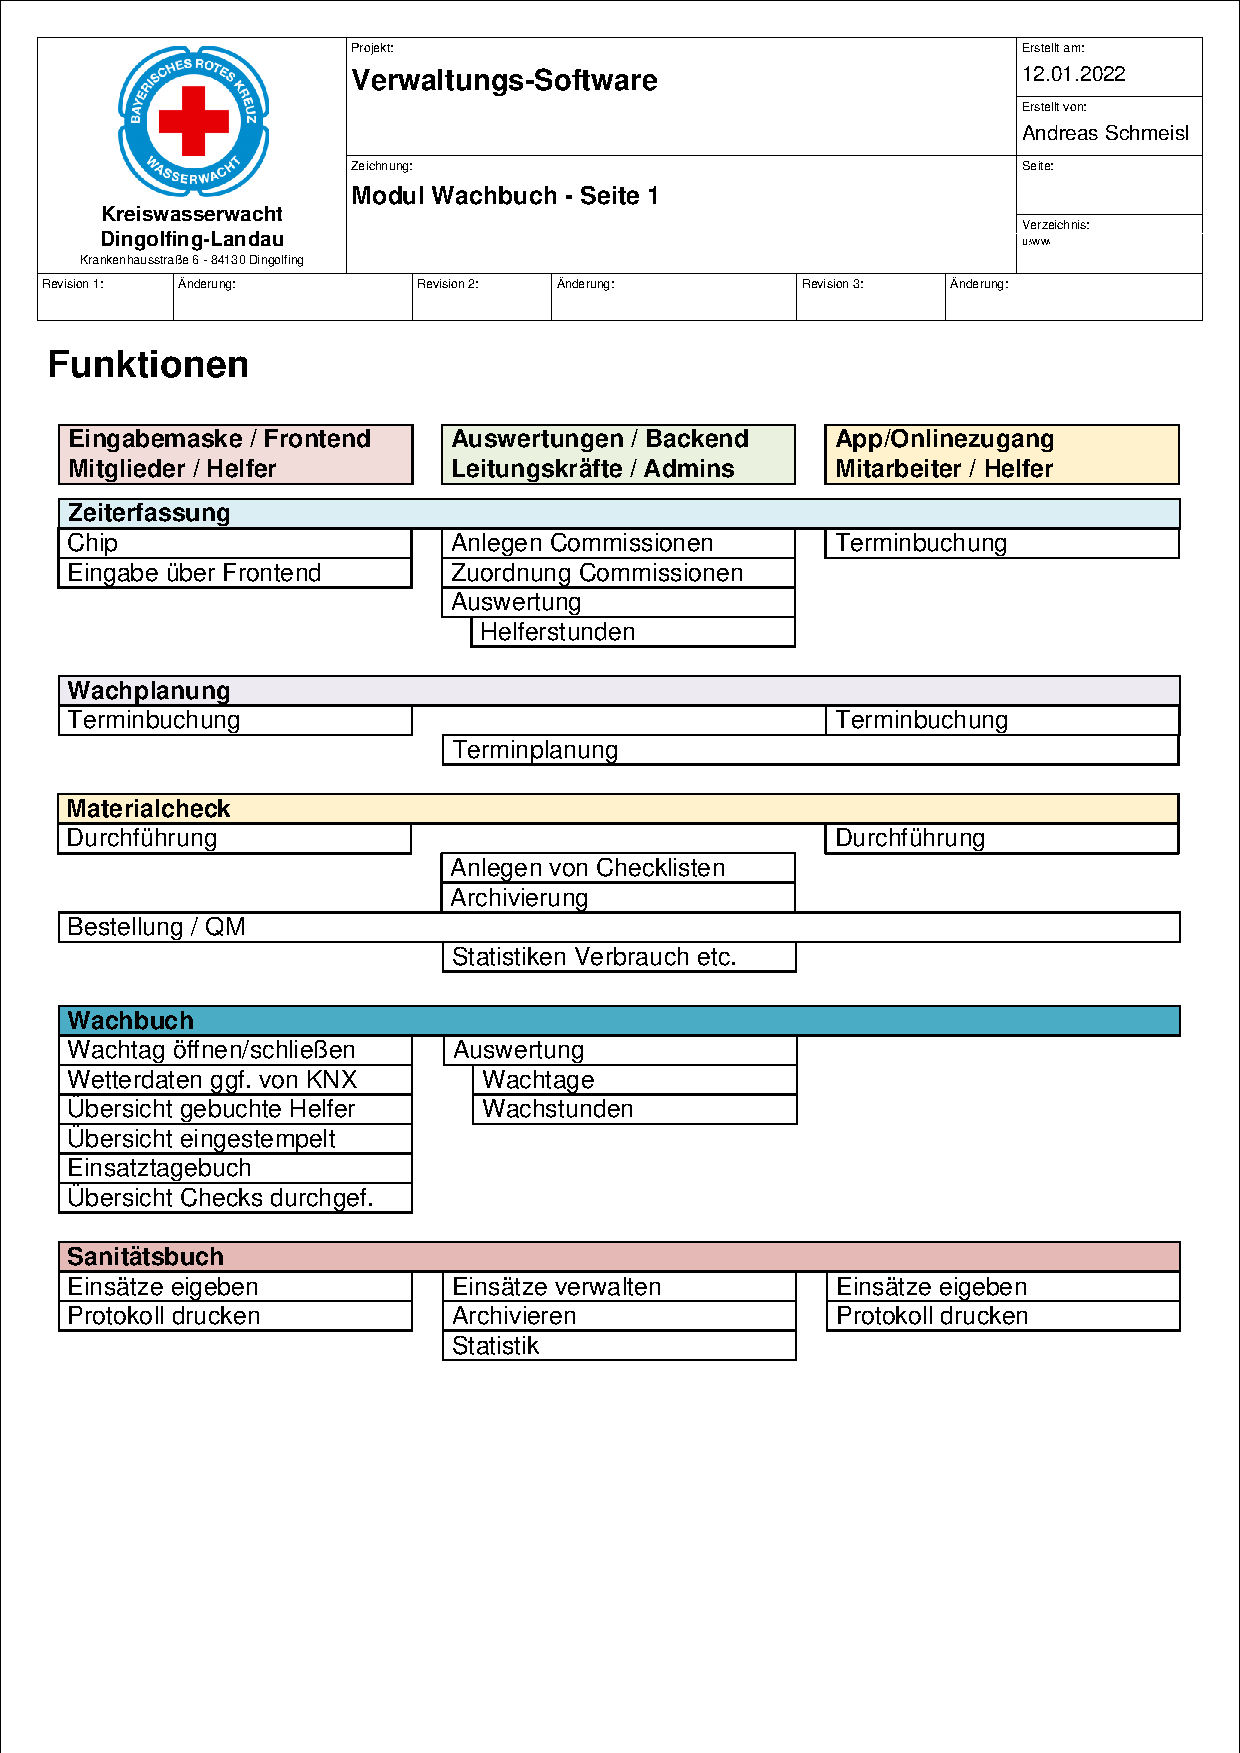
\includepdf[
    pages=1-2,
    frame,
    scale=.75]
    {Anlagen/WSM_Software_Modul_Wachbuch.pdf}
\begin{figure}[H]
\centering
    \includegraphics[page=3,scale=0.75]{Anlagen/WSM_Software_Modul_Wachbuch.pdf}
  \caption{Initialer Entwurf}
  \label{fig:initial}
\end{figure}

\section{Wachbuch Papier}

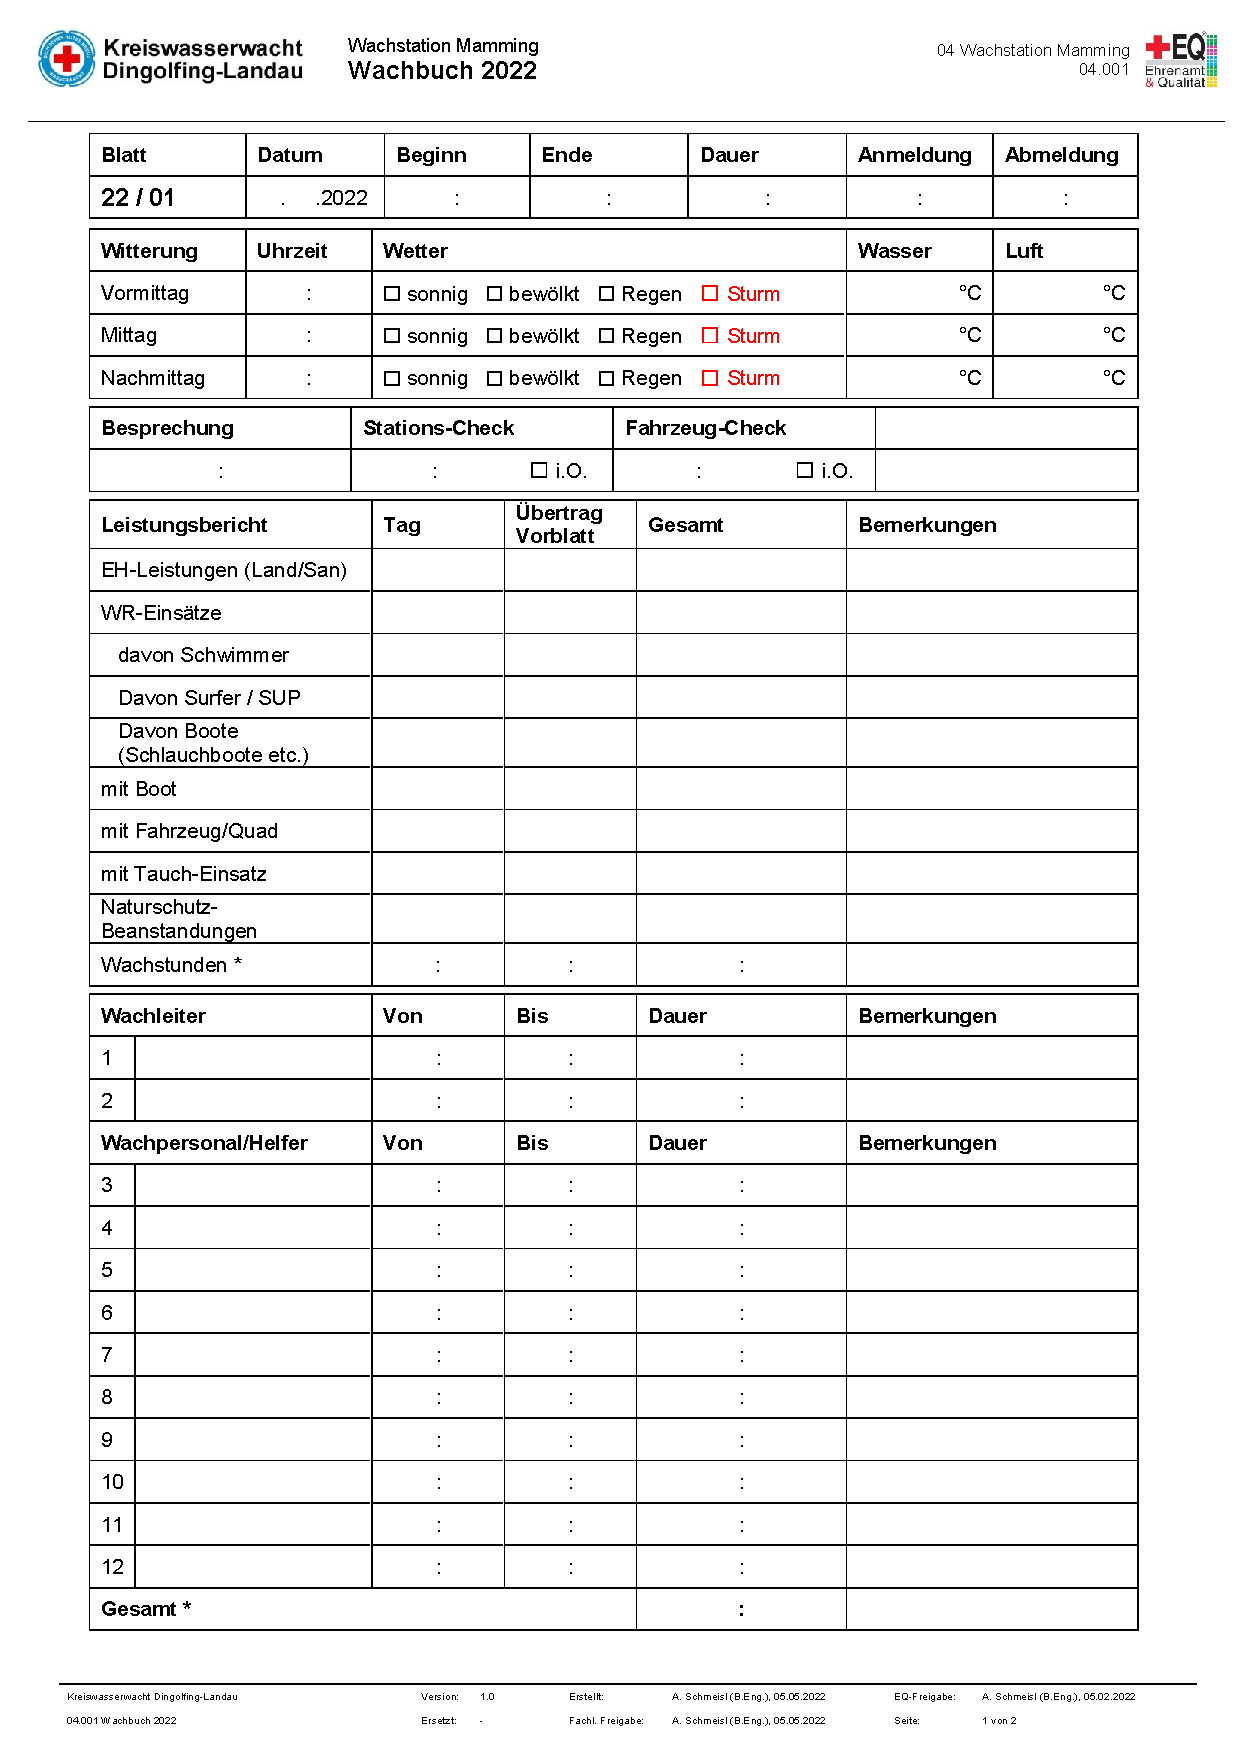
\includepdf[
    pages=1,
    frame,
    scale=.75]
    {Anlagen/wachbuchPapier.pdf}
\begin{figure}[H]
\centering
    \includegraphics[page=2,scale=0.75]{Anlagen/wachbuchPapier.pdf}
  \caption{Wachbuch Papier}
  \label{fig:wachbuchpapier}
\end{figure}


\end{appendix}

	 
% References (Literaturverzeichnis):
\bibliographystyle{alpha}
\bibliography{Literatur}


%%%%%%%%%%%%%%%%%%%%%%%%%%%%%%%%%%%%%%%%%%%%%%%%%%%%%%%%%%%%
\end{document}
